\subsubsection{DataAccess}
DataAccess implementerer IDataAccess og står for at skrive og læse data records til/fra databasen.
IDataAccess refereres af klassen SmartPoolDB. Klassen DataAccess kan ses på figur \ref{fig:dataAccessClassNoInherit}

\begin{figure}
\centering
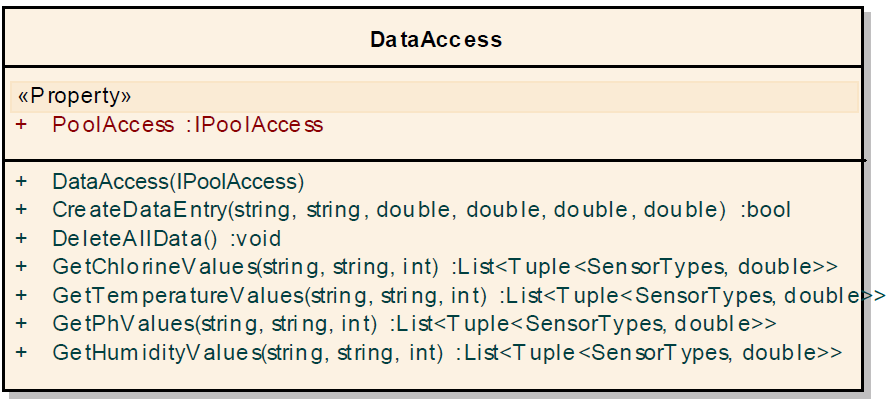
\includegraphics[width=0.7\linewidth]{figs/implementering/dataAccessClassNoInherit}
\caption{Klassen DataAccess}
\label{fig:dataAccessClassNoInherit}
\end{figure}

\paragraph{CreateDataEntry}\ %%%%%%%%%%%%%%%%%%%%%%%%%%%%%%%%%%%%%%%%%%%%%%%%%%%%%%%%%%%%%%%%%%%

\subparagraph{Signatur}
\begin{itemize}
	\item \textit{bool CreateDataEntry(string ownerEmail, string poolName, double chlorine, double temp, double pH, double humidity)}
\end{itemize}

\subparagraph{Returnere:}
\begin{itemize}
	\item \textit{Boolean}, true hvis data kunne sættes ind i databasen uden problemer, ellers false.
\end{itemize}

\subparagraph{Argumenter:}
\begin{enumerate}
	\item \textit{string} email addressen til den bruger, som poolen tilhøre.
	\item \textit{string} navnet på poolen.
	\item \textit{double} klor værdien som skal indsættes.
	\item \textit{double} temperatur værdien som skal indsættes.
	\item \textit{double} pH værdien som skal indsættes.
	\item \textit{double} luftfugtigheds værdien som skal indsættes.
\end{enumerate}

\subparagraph{Virkemåde}
\begin{itemize}
	\item Først tester metoden om brugeren har en pool med det givne navn. Metoden gemmer så tidspunktet og opretter et \textit{Data} object (som vist i figur~\ref{fig:datasetentity}), som gemmes i databasen. Herefter oprettes målingerne og tildeles den fælles \textit{Data} som tidligere blev oprettet.
\end{itemize}

\begin{figure}
\centering
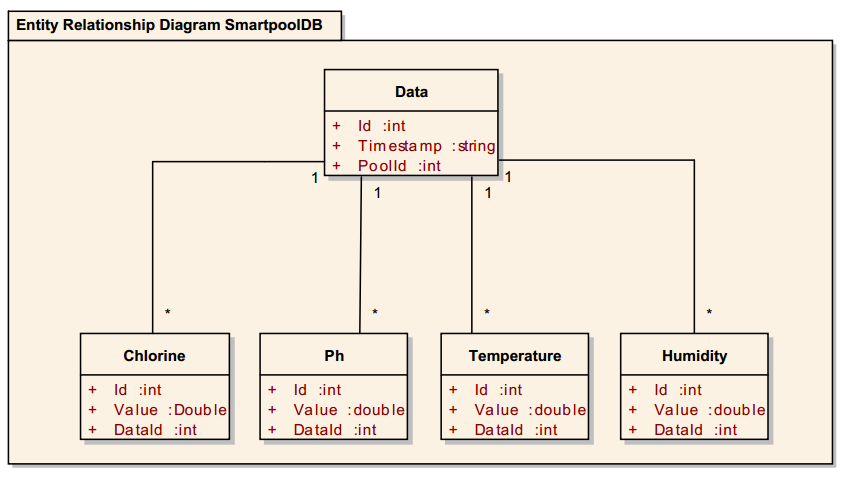
\includegraphics[width=0.8\linewidth]{figs/implementering/datasetentity.png}
\caption{En del af ER diagrammet som databasen er lavet udfra.}
\label{fig:datasetentity}
\end{figure}






\subparagraph{DeleteAllData}\ %%%%%%%%%%%%%%%%%%%%%%%%%%%%%%%%%%%%%%%%%%%%%%%%%%%%%%%%%%%%%%%%%%%







\subparagraph{Signatur}
\begin{itemize}
	\item \textit{void DeleteAllData()}
\end{itemize}

\subparagraph{Returnere:}
\begin{itemize}
	\item \textit{void}.
\end{itemize}

\subparagraph{Argumenter:}
\begin{enumerate}
	\item Tager ikke nogle argumenter.
\end{enumerate}

\subparagraph{Virkemåde}
\begin{itemize}
	\item Lavet til brug under test og udvikling. Rydder tabellerne for Data og målinger (Chlorine, Ph...).
\end{itemize}







\subparagraph{GetChlorineValues}\ %%%%%%%%%%%%%%%%%%%%%%%%%%%%%%%%%%%%%%%%%%%%%%%%%%%%%%%%%%%%%%%%%%%






\subparagraph{Signatur}
\begin{itemize}
	\item \textit{List<Tuple<SensorTypes, double>> GetChlorineValues(string poolOwnerEmail, string poolName, int daysToGoBack)}
\end{itemize}

\subparagraph{Returnere:}
\begin{itemize}
	\item \textit{Boolean}, true hvis data kunne sættes ind i databasen uden problemer, ellers false.
\end{itemize}

\subparagraph{Argumenter:}
\begin{enumerate}
	\item \textit{string} email addressen til den bruger, som poolen tilhøre.
	\item \textit{string} navnet på poolen.
	\item \textit{double} klor værdien som skal indsættes.
	\item \textit{double} temperatur værdien som skal indsættes.
	\item \textit{double} pH værdien som skal indsættes.
	\item \textit{double} luftfugtigheds værdien som skal indsættes.
\end{enumerate}

\subparagraph{Virkemåde}
\begin{itemize}
	\item Først tester metoden om brugeren har en pool med det givne navn. Metoden gemmer så tidspunktet og opretter et \textit{Data} object (som vist i figur~\ref{fig:datasetentity}), som gemmes i databasen. Herefter oprettes målingerne og tildeles den fælles \textit{Data} som tidligere blev oprettet.
\end{itemize}








\subparagraph{GetTemperatureValues}\ %%%%%%%%%%%%%%%%%%%%%%%%%%%%%%%%%%%%%%%%%%%%%%%%%%%%%%%%%%%%%%%%%%%

\textit{List<Tuple<SensorTypes, double>> GetTemperatureValues(string poolOwnerEmail, string poolName, int daysToGoBack)}
\todo{do dis}

\subparagraph{GetPhValues}\ %%%%%%%%%%%%%%%%%%%%%%%%%%%%%%%%%%%%%%%%%%%%%%%%%%%%%%%%%%%%%%%%%%%

\textit{List<Tuple<SensorTypes, double>> GetPhValues(string poolOwnerEmail, string poolName, int daysToGoBack)}
\todo{do dis}

\subparagraph{GetHumidityValues}\ %%%%%%%%%%%%%%%%%%%%%%%%%%%%%%%%%%%%%%%%%%%%%%%%%%%%%%%%%%%%%%%%%%%

\textit{List<Tuple<SensorTypes, double>> GetHumidityValues(string poolOwnerEmail, string poolName, int daysToGoBack);}
\todo{do dis}
